\chapter{Introduction and literature review} \label{sec:intro}


\section{General introduction}

Electrophysiological measurements of neural tissue allow direct observations of millisecond changes in neural activity \cite{Donoghue2020}, on a broad range of spatial scales from micrometers to centimeters. At these large spatial scales, electrophysiological measurements can be made entirely noninvasively through the recording of electrical potentials at the scalp. Over the last century, such scalp recordings, also known as electroencephalography (EEG), have allowed us to measure ongoing neural activity in healthy humans, as well as those suffering from neurological disease, proving itself to be a uniquely important tool for understanding the human brain. Extracting as much information as possible from these signals despite their low spatial resolution is thus highly desirable. Broadly speaking, a fundamental question is: given a difference between two EEG signals, either collected at two timepoints or from two different subjects, how much can we infer about the underlying differences in neurophysiology? 

In general, signals can be narrowband or broadband depending on their frequency profile. A narrowband signal delivers its power within a narrow frequency band, meaning that it can be though of as a signal with a characteristic frequency. A broadband signal exhibits power across a broad range of frequencies and do not have a characteristic frequency. For example, a simple sine wave is a narrowband signal, as it's power spectrum is a delta function at the frequency of oscillation. In contrast, Gaussian noise is a broadband signal, as carries uniform power across all frequencies. However, broadband signals do not need to be white noise. Brownian motion exhibits broadband fluctuations -- the particle's position is not rhythmic, but the majority of power is concentrated at lower frequencies. In fact, its power spectrum following a $1/f^2$ distribution. In reality, complex signals may be comprised of many components, each of which has separate characteristics. 

Starting with the first EEG recordings and Berger’s discovery of the alpha rhythm \cite{Berger1929}, the study of EEG has been synonymous with the study of brain oscillations, and thus EEG is typically considered as a superposition of multiple narrowband signals. ``EEG is a record of the oscillations of brain electric potential.'' So begins the book \textit{Electric fields of the brain: the neurophysics of EEG} by Nunez and Srinivasan \cite{Nunez2006}, the most widely cited reference for EEG theory. However, it is not uncommon that signals in nature exhibit both narrowband and broadband features. 

The fact that the EEG signal has broadband characteristics was noted in 1938 in the very first publication showing EEG spectra, which was computed with a mechanical apparatus of various wheels and projectors to transform the EEG output into Fourier space  (Grass and Gibbs, J. Neurophysiol. 1938). It was noted that ``Inspection of such continuous spectrums should convince one of the inadvisability of referring to certain potentials as alpha, beta, delta waves, etc.''  (Grass and Gibbs, J. Neurophysiol. 1938). This advice was largely ignored (IFSECN working group. Electroencephalography and Clinical Neurophysiology, 1974; https://doi.org/10.1016/0013-4694(74)90099-6), however. After the introduction of computer analysis in the 1960s, EEG spectra became more routinely examined, but the broadband components of these spectra were only ever mentioned in passing. For example, in comparing the EEG spectra of evoked activity between different electrodes, Boudreau and Freeman (Experimental Neurology 1963) noted in 1963 that there was an apparent rotation of the spectrum. The authors hypothesized that this phenomenon could be due to normally-distributed conduction delays between two brain regions, thus effectively low-pass filtering the propagation of activity from one brain region to the other. However, presumably due to the entrenched characterization of EEG as a measure of brain rhythms, it was Freeman’s view that the aim of EEG spectral analysis was the ``disclosure of sinusoidal periodicities buried in the random background activity'' (Freeman. Mass Action in the Nervous System 1975), and deeper examinations of this broadband spectral phenomenon were seemingly never attempted. 

The view that the broadband content in EEG was ``random background activity'' to be discarded or ignored reflects the prevailing sentiment of the time, as it was not until the 1990s that Pritchard (Inter. J. Neurosci 1992) considered the EEG spectral trend as a feature in its own right. In his paper, Pritchard argued that EEG spectra exhibit power law scaling and thus that the brain is fractal in nature, a claim that effectively kickstarted multiple competing theories on the origin and meaning of the background EEG spectrum (\autoref{sec:theories}). Is the EEG spectral trend noise? Or does it reflect something interesting about the brain activity? Does it affect measurements of brain rhythms? 

This final question has become particularly salient in recent years with the publication of Donoghue et al. \cite{Donoghue2020}. In their technical report, a user-friendly algorithm was presented for decomposing EEG into periodic components (i.e. brain rhythms) and a $1/f^\beta$ component -- in line with Pritchard's argument that the trend follows a power law. This algorithm stimulated a flurry of studies linking changes in the extracted 1/f component and the spectral exponent, $\beta$, to cognition, aging, neurological disorders, and altered states of consciousness. However, because this analysis technique is phenomenological in nature, interpreting differences in the 1/f component has been speculative, and the veracity of detrended EEG analyses remains debatable. These recent developments highlight a pressing need for a theory of aperiodic EEG that is physiologically grounded and practically applicable.

I will go into these various theories in depth towards the end of this Introduction, but for now, what exactly do we mean by broadband EEG and the spectral trend?

\newpage

\section{Spectral trend observed in macroscopic neural recordings} \label{sec:phenomenon}

\section{The biophysics of EEG} \label{sec:EM_theory}

A major benefit of EEG, and electrophysiological measurements in general, is that the biophysics of these measurements are well understood. In this section, I review the basics of electromagnetism in a volume conductor and build up to forward models of the EEG -- models that take a distribution of currents in the brain and give as an output the electric potential at the scalp.

\subsection{Maxwell's equations and the electric potential}
In 1873, James Clerk Maxwell published \textit{A treatise on electricity and magnetism}, accomplishing for electromagnetism what Newton had for mechanics. In four equations, the behaviour of all classical phenomena related to electricity and magnetism could be described. As such, they are what allow us to take physiology and form theories on electrophysiology. The equations are
\begin{align*}
    & \nabla \cdot \bm{E} = \frac{\rho}{\epsilon_0} \\
    & \nabla \cdot \bm{B} = 0 \\
    & \nabla \times \bm{E} = - \frac{\partial {B}}{\partial t} \\
    & \nabla \times \bm{B} = \mu \left( \bm{J} + \epsilon_0 \frac{\partial \bm{E}}{\partial t} \right)
\end{align*}
Here, $\bm{E}$ is a vector field called the electric field and $\bm{B}$ is a vector field called the magnetic field. The first two equations describe the divergence of these fields and the latter two equations describe the curl of these fields. 

The first equation states that the sources (positive divergence) and sinks (negative divergence) of the electric field are electric monopoles, otherwise called an electric charge. $\rho$ is the density of charge at each point in space and when scaled by $\epsilon_0$, the permittivity of a vacuum, one gets the divergence of the electric field. Negative charges are sinks of the electric field and positive charges are sources of the electric field. The second equation states that there are no source or sinks of the magnetic field. In other words, there are no magnetic monopoles. The third and fourth equation describe how the electric and magnetic field interact with each other. The third equation is called the Faraday's law of induction and describes how a time varying magnetic field can induce an electric field. The final equation is Ampère's law and describes how a magnetic field is generated by either an electric current or a time varying electric field.

\subsubsection{The quasi-stationary approximation of the electric potential}
In EEG, the electromagnetic field can be assumed to be static which is called the quasi-stationary approximation (Plonsey and Heppner, Bulletin of Mathematical Biophysics, 1967). This approximation is valid because the frequencies of EEG we are interested in (less than \qty{1}{\kilo\hertz}) are slow compared to the timescale of interactions between the electric and magnetic fields \cite{RevModPhys.65.413}. As a result of the assumption, all the time derivatives in the equations are zero, reducing Maxwell's equations to
\begin{align}
    & \nabla \cdot \bm{E} = \frac{\rho}{\epsilon_0} \\
    & \nabla \cdot \bm{B} = 0 \\ 
    & \nabla \times \bm{E} \approx 0 \label{eq:QSA_induction} \\ 
    & \nabla \times \bm{B} \approx \mu \bm{J} \label{eq:QSA_amp_law}
\end{align}
Notice that the electric field has become uncoupled from the magnetic field. This assumption allows for valid and (relatively) simple calculations of the electric potential at the scalp.

\subsubsection{Calculating the electric potential at the scalp}
EEG electrodes measure the electric potential, $\phi$, at a location on the scalp. The electric potential of an electric field is defined by the fundamental theorem of vector calculus: $\bm{E} = - \nabla \phi + \nabla \times \bm{A}$, where $\bm{A}$ is some divergence-free vector field. Under the quasi-stationary approximation, the electric field has no curl (\ref{eq:QSA_induction}), and thus $\nabla \times \bm{A}$ must equal zero, simply giving us that 
\begin{equation} \label{eq:potential}
\bm{E} = -\nabla \phi
\end{equation}
This equation tells us that the electric field is entirely defined by the gradient of the electric potential. We can therefore calculate the electric potential from its relationship with the electric field. To do so, we make use of two additional relationships.

First, an electric field in a conductor acts on free charges and gives rise to a passive current that obeys Ohm's law. That is, $\bm{J}^{passive}(\bm{r}) = \sigma(\bm{r}) \bm{E}(\bm{r})$, where $\sigma$ is the macroscopic conductivity. This equation can be very general \cite{Pettersen2012}: $\sigma$ may be a tensor, meaning that the conductivity varies depending on the direction (anisotropy), it may be complex to account for capacitive effects, and it may be frequency dependent, in which case the above multiplication becomes a convolution. This latter case does not seem to be relevant for EEG, but see \autoref{sec:filter_theory} below.

Second, the total current is equal to this passive current plus the primary currents, $\bm{J}^p(\bm{r})$, i.e., those arising from synaptic transmission, action potential firing, etc. This decomposition is expressed as $\bm{J}(\bm{r}) = \bm{J}^p(\bm{r}) + \sigma(\bm{r}) \bm{E}(\bm{r})$. Now, we take the final step in the derivation. We can take the divergence of both sides of \ref{eq:QSA_amp_law}, and because the divergence of the curl is zero, we get that $\nabla \cdot \bm{J} = 0$. Thus, substituting in \ref{eq:potential}, we arrive at the Poisson equation describing the electric potential
\begin{equation} \label{eq:poisson}
    \nabla \cdot \bm{J}^p = \nabla \cdot \left(\sigma \nabla \phi \right)
\end{equation}
Note that the air around the scalp is considered to be a perfect insulator, and therefore the boundary condition at this interface is such that there is no current flow normal to the scalp.

In conclusion, we can calculate the difference in electric potential between two electrodes as \cite{RevModPhys.65.413}
\begin{equation}
    \phi_i(t) = \int_V \mathcal{L}_i(\bm{r}) \cdot \bm{J}^p(\bm{r}) dV(\bm{r})
\end{equation}
where $\mathcal{L}_i$ is called the lead field for the $i$th lead  and describes the sensitivity of the potential to currents sources at each location in space \cite{Malmivuo1995}.

\subsection{The multipole expansion and current dipoles} \label{sec:dipoles}
The potential due to all current sources in a medium can be expressed as a so-called multipole series expansion \cite{Nunez2006}. The first term is the \textit{monopole} contributions, which are the contributions of all isolated current sources and sinks. The second term is the contributions from current \textit{dipoles}, which are paired current sources and sinks of equal magnitudes separated by an infinitesimal distance. Due to this specific arrangement, the currents cancel out and thus the dipole has no net monopole moment. The third term is the \textit{quadruple} contribution. Analogous to the dipole, the quadruple is the arrangement of four currents that together have no monopole nor dipole moment. These first three terms of the multipole expansion are illustrated in \autoref{fig:multipole}. 

\begin{figure}[t!]
	\centering
	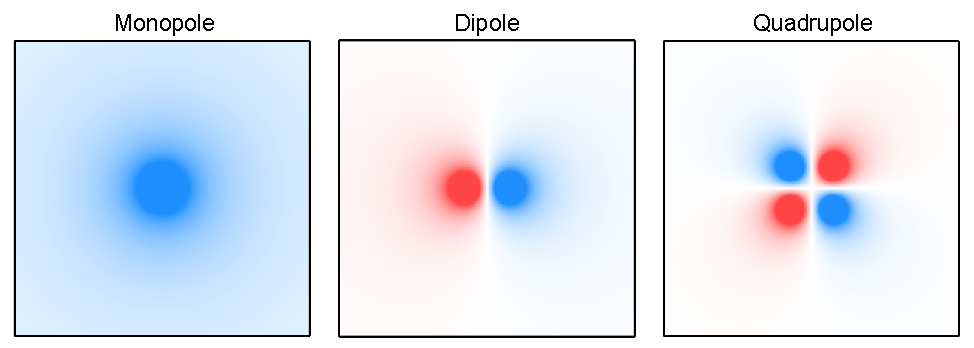
\includegraphics[width=\textwidth]{Figures/chapter1/multipole_expansion.pdf}
    
    \caption{\textbf{Illustration of the first three terms of the multipole expansion.} \textbf{Left}: The current monopole corresponds to the net flow of current into or out of a volume and is equal in all directions. \textbf{Middle}: The current dipole incorporates two equal and opposite monopoles separated by an infinitesimal distance. Thus, the net current associated with these monopoles cancel out. Instead, dipoles express the directionality of current flow. In this illustration, the dipole is horizontally oriented. \textbf{Right}: The quadrupole incorporates two equal and opposite dipoles. Like the dipoles, there is no net current flow. Moreover, the directions of the dipoles cancel out, and therefore there is also no directionality. } 
    \label{fig:multipole}
\end{figure}

The contribution of each pole to the electric potential decreases with distance at a different rate \cite{Nunez2006}. Specifically,
\begin{equation}
    \phi(R) = \frac{C_{monopole}}{R} + \frac{C_{dipole}}{R^2}  + \frac{C_{quadrupole}}{R^3}  + ...
\end{equation}
The sources and sinks of current are balanced throughout the brain and thus for electric fields generated by macroscopic volumes of tissue, the monopole term is approximately zero \cite{Nunez2006}. Furthermore, for electrodes far away from the current densities, as is the case for EEG, the higher orders terms contribute negligibly relative to the lower order terms. Consequently, EEG signals can be accurately modelled based on current dipoles alone \cite{Nunez2006,RevModPhys.65.413}. This gives us the following equation for the EEG signal \cite{RevModPhys.65.413}
\begin{equation} \label{eq:lead_solution}
    \phi_i(t) \approx \int_V \mathcal{L}_i(\bm{r}) \cdot \bm{Q}(\bm{r},t) dV(\bm{r})
\end{equation}
where $\bm{Q}$ is the current dipole moment at point $\bm{r}$ in the brain. From this equation, it is clear that after knowing the distribution of current in the brain, the difficulty in modelling EEG signals comes from defining the lead field, $\mathcal{L}_i(\bm{r})$, at each point in the brain. This lead field must take into account the distribution of conductivity, $\sigma(\bm{r})$, so that the effects of volume conduction are properly modelled. The assumptions that go into calculating $\mathcal{L}_i(\bm{r})$ are together called a head model, i.e., a model that encapsulates all the effects of the head on volume conduction (\autoref{sec:head_models}).

\subsection{Physiological basis of current dipoles}
Compared to the biophysics of EEG, the neural basis of EEG remains surprisingly mysterious. As described in the previous section, the primary generators of EEG signals are current dipoles in the brain (\autoref{sec:dipoles}). So what in the brain causes these current dipoles? The short answer is ion channels: pores in cell membranes that transport ions down their concentration gradient. In theory, all ion channels, from glutamate receptors, to voltage-gated sodium channels, to nonspecific ``leak'' channels contribute to the EEG signal \cite{Buzsaki2012}. Even though neurons only make up about half the cells of the brain \cite{Azevedo2009}, their transmembrane current constitute the primary sources of EEG \cite{Buzsaki2012}.

\subsubsection{Passive ion channels}
At rest, the membrane potential of neurons is hyperpolarized to anywhere between -80 and \qty{-50}{\milli\volt} \cite{Ren2011}. This level is approximately described by the Goldman-Hodgkin-Katz equation \cite{Hodgkin1949} and depends on the internal and external concentration of potassium, sodium, and chloride ions, as well as the membrane's permeability to each. At rest, the primary membrane conductances are through a large family of two-pore potassium channels \cite{Goldstein2005,Ren2011} which are non-voltage-gated, outwardly rectifying potassium channels \cite{Goldstein2001}. The Nernst potential for potassium is around \qty{-90}{\milli\volt}, so given that the resting membrane potential is more depolarized than this, there must also be some sodium leak current. Indeed, it has been discovered relatively recently that this sodium leak is provided by the channel NALCN (Na\textsuperscript{+} leak channel, non-selective) \cite{Ren2011}. Together, these sodium and potassium leak currents are the primary determinants of the resting membrane potential of the cell. In biophysical modelling, all these leak currents are often lumped together into a single leak conductance with a reversal potential defined as the resting membrane potential (often around \qty{-65}{\milli\volt}). These passive ion channels flux currents that slowly restore the membrane potential following excursions.

\subsubsection{Ligand-gated ion channels}
Chemically-gated ion channels are the primary means by which neurons communicate with one another. While there are ion channels that are coupled to receptors for most neurotransmitters, the vast majority of neuronal communication occurs through iontropic glutamate and GABA receptors. Iontropic glutamate receptors fall into four classes, AMPA, NMDA, kainate, and GluD receptors, of which AMPA and NMDA receptors are the best understood \cite{Hansen2021}. Both channels are expressed predominantly at postsyanptic sites, although both can also be found extrasynaptically \cite{Clark2002,Lin2009}. Glutamate is released by the presynapatic neuron into the synaptic cleft, where it lingers for a couple milliseconds \cite{Clements1992}. During this time, glutamate binds the ligand-binding domain of AMPA receptors, opening a non-specific cation channel that depolarizes the postsynaptic membrane potential. The dissociation kinetics of AMPA receptors is relative fast, meaning that the channel shuts down shortly after glutamate is cleared from the synaptic cleft, producing a transient depolarizing current that lasts anywhere from $<$\qty{1}{\millsecond} to \qty{8}{\millsecond} depending on the deactivation kinetics of the specific molecular composition of the AMPA receptor complex \cite{Geiger1997,Howe2015,Greger2017}. NMDA receptors hold on to glutamate much longer and thus producing long lasting currents up to several tens of milliseconds. However, unlike AMPA receptors, NMDA receptors have voltage-sensitive channels and only pass current if the postsynaptic membrane potential is already sufficiently depolarized. 

\subsubsection{Voltage-gated ion channels}

\subsection{Source current models}
Historical, modellers have considered mesoscopic dipoles.

Naess and the single neuron dipoles...


\subsection{Head models of volume conduction} \label{sec:head_models}
There are many models that may be used in forward EEG modelling. The simplest is to assume that we are measuring the electric potential inside an infinite, homogeneous volume conductor. Under this assumption, the electric potential at a point $\bm{r}^\prime$ generated by a dipole at a point, $\bm{r}$, is given by
\begin{equation}
    \phi = \frac{\bm{d} \cdot \bm{Q}}{4\pi\sigma |\bm{d}|^3}
\end{equation}
where $\bm{d}=\bm{r}^\prime-\bm{r}$. This equation should be recognizable as it is very similar to Coulomb's law for the electric field generated by static charges. This model is fairly reasonable for modelling LFP \cite{Pettersen2012}, but it is a gross simplification for modelling EEG, as it neglects the large differences in conductivity between neural tissue, the scalp, and the skull.

To capture this variation in conductivity, a popular model is the concentric spheres model. Under this model, the head is composed of concentric spherical layers of different radii and conductivity \cite{Geisler1961}. In the most accurate, four-sphere model \cite{Hosek1978}, the layers represent from inside out: the brain, cerebral spinal fluid, skull, and scalp. The major benefits of these models are that they (i) are more accurate than the infinite, homogeneous volume conductor model, and (ii) can be solved analytically, although the solutions are mathematically and notationally complex. A complete derivation and numerically validated solution to the four-sphere model is given Næss et al. \cite{Næss2017}.

After the analytical solutions, the most accurate models rely on numerical solutions to the Poisson equation (\ref{eq:poisson}) using techniques such as the finite element method. In this method, the problem domain is meshed into discrete ``elements'' within each of which the solution can be approximated by a simple, e.g., linear, function \cite{Liu2014}. In head modelling, this typically means representing the various tissues of the head with a mesh of tetrahedral elements with different conductivity \cite{Hallez2007}. An example two-dimenisonal mesh of a coronal section of the head is shown in \autoref{fig:FEM_mesh}A. Notice that the density of the mesh changes and becomes denser close to the interfaces of different tissue types. The larger the gradient of the electric field, the denser the mesh needs to be for accurate solutions. After this meshing procedure, the entire system can be represented by a sparse matrix, where each element is characterized by its approximate linear function and is connected to its adjacent elements.

\begin{figure}[t!]
    \centering
    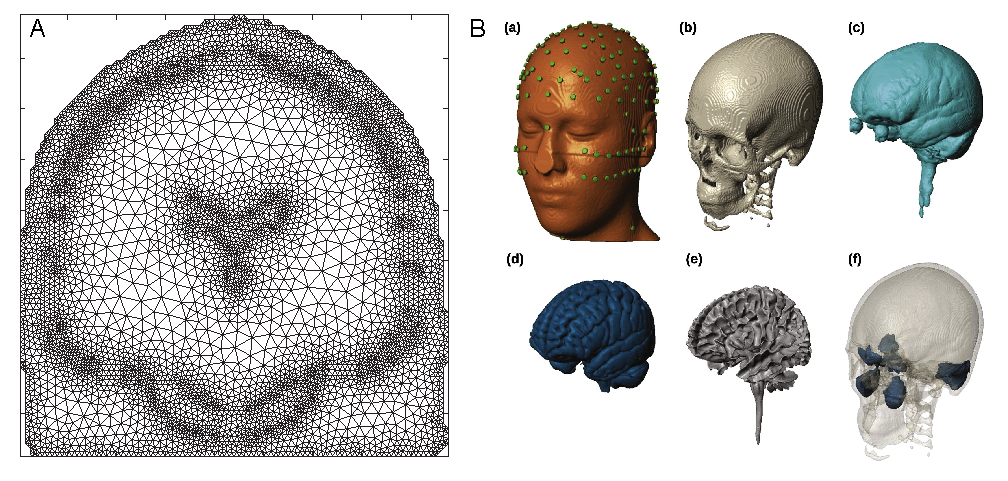
\includegraphics[width=\textwidth]{Figures/chapter1/FEM_mesh.pdf}
    
    \caption{\textbf{Head models using the finite element method.} 
    (\textbf{A}) Example triangular mesh of a coronal section of the head used for finite element modelling. Figure adapted from Hallez et al. \cite{Hallez2007} under a Creative Commons license. © 2007 Hallez et al; licensee BioMed Central Ltd. (CC BY 2.0).
    (\textbf{B}) Segmentation of head model into six tissue types: scalp (\textbf{a}), skull (\textbf{b}), cerebro-spinal fluid (\textbf{c}), gray matter (\textbf{d}), white matter (\textbf{e}), and air cavities (\textbf{f}). The location of 231 electrodes are shown on the scalp in panel (a). Figure adapted from Huang et al. \cite{Huang2016} under a Creative Commons license. © 2016 Huang et al (CC BY 4.0).
    } 
    \label{fig:FEM_mesh}
\end{figure}

Computing the lead field with the finite element method is computational intensive and not practical for every individual. Therefore, head models are typically based on a the heads of a single, representative individual \cite{Holmes1998}. An improvement over this was introduced with the the New York Head model \cite{Huang2016}. In this model, Huang et al. constructed a mesh of the ICBM152 anatomical template, which is an average MRI of 152 subjects, and included six different tissue types: scalp, skull, cerebral spinal fluid, gray matter, white matter, air cavities (\autoref{fig:FEM_mesh}B). Therefore, this head model represents an average head and may thus be more generalizable.  This head model computed the lead field, $\mathcal{L}_i(\bm{r})$, for 231 electrode locations ($i\in\{1,2,...,231\}$) and for  ${\sim}75000$ cortical locations ($\bm{r}\in\{ \bm{r}_1, \bm{r}_2, ..., \bm{r}_{74382} \}$). These lead fields can be precomputed and stored, thus allowing high accuracy solutions to the forward EEG problem with low computational costs.


\section{The standard model of EEG} \label{sec:standard_model}

\subsection{Synchrony of synaptic currents}
In addition to the biophysics of EEG generation, there are two key neural features important for EEG generation: geometry and dynamics. In order to generate electric fields large enough to be detected at the scalp, ion channels must be generating current dipoles that are coherent \cite{Buzsaki2012, Nunez2006}, and because dipoles are vectors, this means that both the temporal dynamics and the spatial configuration of these dipoles must be correlated.

Based on early experimental observations of how superficial potentials propagate following cortical simulation, mid-century electrophysiologists \cite{Eccles1951} reasoned that the EEG signal is likely generated by excitatory synaptic inputs onto the apical dendrites of pyramidal neurons (\autoref{fig:eccles}). This was controversial at the time, as others still believed that the signal primarily reflected action potentials \cite{Burns1950}. It was later confirmed through cross-correlation analysis that postsynaptic potentials and the EEG signal are statistically related \cite{KLEE1965}. Broadly, the synaptic current model became the canonical viewpoint and notably provides both of the necessary mechanisms for EEG generation: (i) synaptic currents last longer than action potential and therefore overlap more in time, which increases the chance of a superposition of current dipoles; and (ii) because of the parallel orientation of pyramidal neurons, synchronized synaptic input into their apical dendrites should generate similarly oriented dipoles.

\begin{figure}
  \begin{minipage}[c]{90mm}
    \includegraphics[width=\textwidth]{Figures/chapter1/Eccles_1951.png}
  \end{minipage}\hfill
  \begin{minipage}[c]{75mm}
    \caption{ \captiontitle{Detectable EEG signals require only weak, locally synchronized dipoles.}
    Diagram by Eccles. 
    Reprinted from Electroencephalography and Clinical Neurophysiology, Vol 3/4, J.C. Eccles, Interpretation of action potentials evoked in thecerebral cortex, Pages No. 449-464, Copyright (1951), with permission from Elsevier.
    \vfill
    } \label{fig:eccles}
    
  \end{minipage}
\end{figure}

Early work debated whether EEG signals reflected just excitatory postsynaptic potentials or additionally inhibitory postsynaptic potentials (Pollen. EEG Clin. Neurophysiol. 1964; Creutzfeld et al. EEG Clin. Neurophysiol. 1965). Typically, inhibitory synapses are thought to be primarily concentrated on the somatic compartments, and therefore do not generate as large dipoles as the distally placed excitatory synapses. Furthermore, the reversal potential of GABA receptors is closer to the resting membrane potential of the cell, and it has thus been argued that they do not generate as large currents. 

However, neither of these arguments are entirely true. Firstly, inhibitory cells do in fact target the apical dendrites of pyramidal neurons, and while there is a high density of inhibitory synapses on the soma and axon initial segment, whole-cell synapse mapping shows that the distribution of inhibitory synapses is more or less uniform across the entire dendritic arbour \cite{Iacaruso2017}. Secondly, in vivo neurons are constantly bombarded by excitatory and inhibitory synaptic input, meaning that their membrane potential is not at ``rest'' as it is in vitro \cite{Destexhe2003}. The driving force of GABA and AMPA receptors during this high conductance state is much more balanced than in vitro experiments. As such, it is general considered now that both excitatory and inhibitory synaptic currents contribute to EEG signals \cite{Buzsaki2012}. Nonetheless, many studies of network dynamics only consider the excitatory synaptic currents when modelling the EEG signal \cite{Jensen2005,McCarthy2008}, and the relative contribution of these two types of currents to EEG signals is far from established. In sum, although every transmembrane current contributes to extracellular potentials, typically only currents mediated by AMPA (and sometimes GABA) receptors are considered as the generators of EEG rhythms.

\subsection{Synchrony through rhythmicity}
If neurons are all firing randomly, then it does not matter how long synaptic currents last -- the signals are not going to sum together in any appreciable way and no EEG signal will transpire. Enter brain rhythms. Neurons are fundamentally oscillators \cite{HODGKIN1952} and oscillators like to synchronize \cite{Strogatz2015}. In fact, it is often difficult to \textit{stop} coupled oscillators from synchronizing \cite{Erb1992}. It is perhaps not surprising therefore that the brain exhibits synchronized oscillations of neurons. These oscillations in turn produce synchronized postsynaptic currents in large pyramidal cells, giving rise to detectable oscillations on the EEG. This is the so-called ``standard model'' of EEG \cite{Cohen2017}. However, there is nothing standard about the wide range of frequencies, neural assemblies, and synchronizing mechanisms that characterize the repertoire of neural oscillations observed in the brain.  There is an extensive literature on neural oscillations, but in this thesis brain rhythms appear principally as a foil to the broadband EEG component discussed in the next section. Therefore, the following summary of the mechanisms underlying neural oscillations will be a terse one.

The first brain rhythm that was observed was the alpha rhythms (8 to \qty{12}{\hertz}) \cite{Berger1929}, which appears during idleness \cite{Adrian1934}; however, the rhythm may in fact reflect an active inhibition of non-task relevant areas \cite{Cooper2003}. The next rhythms that became apparent are those that are observed during sleep \cite{Loomis1937,Weber2016} and general anesthesia \cite{GIBBS1937,Akeju2017}. Both states share the appearance of delta oscillations ($<4$ \unit{\hertz}), although this rhythm may be caused by distinct underlying mechanisms in sleep and anesthesia \cite{Akeju2017}. Then, there are the rhythms that have been linked to information processing and cognition in awake, behaving humans, including the beta (15 to \qty{30}{\hertz}) \cite{Spitzer2017} and gamma rhythms (30 to \qty{50}{\hertz}) \cite{JASPER1938,Fries2009}. While alpha, beta, gamma, and delta rhythms are perhaps the most notable, there are in fact many more rhythms that have been observed and which span almost the entire frequency range from \qty{0.1}{\hertz} up to \qty{300}{\hertz} \cite{Penttonen2003}. To highlight the diversity in neural rhythms, I will briefly review the neural mechanisms thought to underlie just two of these rhythms: the delta rhythm during sleep and the gamma rhythms observed during wakefulness.

\subsubsection{Example 1: delta rhythms}
Delta rhythms are an intrinsic oscillation of thalamocortical neurons. When these neurons are hyperpolarized to levels below $-65$ to $-70$ \unit{\milli\volt} in vivo, the cells switch from a tonic firing to a bursting regime with a frequency between 0.5 and \qty{4}{\hertz} \cite{Dossi1992}. This bursting activity is characterized by subthreshold oscillations reflecting the interplay of a non-inactivating, hyperpolarization-activated inward current, the h-current, and a low-voltage activated calcium current, the t-current \cite{McCormick1990,Soltesz1991}. These thalamocortical neurons make reciprical connections with the inhibitory reticular thalamic neurons and this population-level negative feedback is thought to synchronize the oscillations of each thalamocortical neuron \cite{Steriade1991, Steriade1993}. In the waking state, input from the active cholinergic system depolarizes the membrane potential of thalamocortical neurons out of the range of bursting and prevents delta oscillations \cite{Steriade2003}. However, during non-REM sleep, the acetylcholine system is suppressed \cite{Watson2010}, and the resulting lack cholinergic input from the brainstem onto thalamocortical neuron is thought to hyperpolarize the thalamocortical neurons into their bursting regime \cite{Steriade2003}. Ultimately, this thalamocortical rhythm produces synchronized excitatory synaptic currents in the cortex, giving rise to the delta oscillations on the EEG during non-REM sleep \cite{Amzica1998}.

\subsubsection{Example 2: gamma rhythms}
 Gamma rhythms have been most completely described in the hippocampus and visual cortex, where it can be evoked by spatial exploration \cite{Bragin1995} and visual attention \cite{Gray1989}, respectively. Unlike the delta rhythm explained above, the gamma rhythm is not an intrinsic property of the constituent neurons. Also unlike the delta rhythm, the gamma rhythm is generated entirely intracortically \cite{Gray1989} and can be examined in vitro using acute cortical slices \cite{Whittington1995}. Such slice work revealed that, mechanistically, gamma oscillations only require a population of reciprocally connected interneurons receiving sufficient excitatory drive \cite{Whittington1995, Buzski2012b}. Indeed, blocking GABA\textsubscript{A} receptors universally prevents gamma oscillations in slices \cite{Bartos2007}. Computational network models validated that networks of interneurons synchronize into a gamma rhythm by virtue of their synaptic decay timescales \cite{Wang1996}. It was thus argued that interneuron gamma oscillations create coherent, subthreshold oscillations in pyramidal neurons that in turn synchronize their excitatory outputs, leading to a gamma oscillations on the EEG \cite{Wang1996}. There is also a model of gamma oscillations that requires excitatory connection, the so-called E-I model, as opposed to the foregoing I-I model \cite{Buzski2012b}. In this model, oscillations are generated by alternating excitatory firing followed by delayed reciprocal inhibition \cite{Borgers2003}. This model is also supported by experimental evidence. For example, depending on the pharmacological intervention used to excite interneurons in a slice, blocking AMPA receptors can also prevent gamma oscillations \cite{Bartos2007}. Regardless of the model, it is agreed that gamma oscillations emerge from the local interactions among cortical neurons \cite{Bartos2007, Buzski2012b}.

\subsection{Summary}
In the standard model, EEG reflects populations of excitatory neurons entrained to an oscillation, by virtue of which their postsynaptic excitatory currents cohere and generate widely correlated current dipoles. The mechanisms that produce synchronous oscillations in neurons are diverse and the spatial scale over which this synchrony is exhibited can vary from patches of the cortex to the entire thalamocortical system. 

\section{Existing theories on the spectral trend} \label{sec:theories}

\subsection{Theory 1. Local versus global synchrony: the classical view} \label{sec:all_oscillations}
The first theory on the EEG spectral trend follows in the tradition of the standard model of EEG and argues that the EEG only reflects brain rhythms; therefore, the spectral trend must reflect an organization of the brain rhythms. 

The idea of neural oscillations has since established its home in the theories of neural information processing through the open window of temporal coding – the concept that neurons, or assemblies of neurons, encode information through the precise timing of action potentials. Although it has been hotly debated whether the brain operates through a temporal code at all, it seems clear that neural synchrony would be highly beneficial for implementing a temporal code in the brain. Consistent with such a functional role, synchronous neural oscillations have been associated with cognitive functions such as object recognition and context-dependent sensory processing (Singer. Annu. Rev. Physiol. 1993; Uhlhaas and Singer. Neuron 2006; Engel et al. Nat Rev Neurosci. 2001). However, theories have also gone further suggesting that brain oscillations are the fundamental architecture supporting generalized brain function (Buszaki Rhythms of the Brain 2006; Buzsáki. Neuron 2010; Buzsáki. Dialogues Clin Neurosci. 2012). The first theory of broadband EEG reviewed here follows in the tradition of temporal coding, namely that the brain operates through the transient synchronization of neural assemblies, that this synchrony occurs through oscillations, that EEG reflects synchronized activity, and thus that EEG signals reflect brain oscillations. In short, EEG signals, even if apparently broadband, are still fundamentally a reflection of oscillatory brain activity. So, how might brain oscillations generate broadband EEG signals? The argument in favour is built upon three pillars.

First, while certain oscillations are often discussed in the context of cognition, such as beta and gamma oscillations, a wide and diverse repertoire of oscillations have been observed in the brain. Slow EEG oscillations with frequency below 1 Hz are apparent during sleep (Achermann and Borbély, Neuroscience 1997), and are likely caused by synchronous oscillations among reticular thalamic and thalamocortical neurons (Steriade et al. J. Neurosci. 1993a, 1993b). On the other end of the scale, ultra-fast oscillations from 200 to 600 Hz were found in the local field potential of the somatosensory cortex of sleeping rats (Kandel and Buzsáki. J. Neurosci. 1997), and also appear in human EEG, particularly in patients with epilepsy (Frauscher et al. Epilepsia 2017). A systematic review from 2003 found brain oscillations that cover the entire range of frequencies between these two extremes (Pentoonen and Buzsáki, Thalamus Relat. Cyst. 2003). Moreover, these oscillations formed a geometric progression whereby lower frequency oscillations, such as delta rhythms, which range from say 1.5-4 Hz, cover a range of a couple Hz, while high frequency oscillations, ranging from 200 to 600 Hz, cover a range of several hundred (Pentoonen and Buzsáki, Thalamus Relat. Cyst. 2003). Consequently, on a logarithmic frequency scale, oscillations provide continuous and linearly spaced coverage with little overlap (Pentoonen and Buzsáki, Thalamus Relat. Cyst. 2003). 

Second, it is thought that slower oscillations recruit larger assemblies of neurons that faster oscillations. Conceptually, it has been argued that, due to conduction delays, communication among spatially broad ensembles of neurons must have more tolerance in signal timing (“obtaining a global consensus takes more time”), and are therefore organized into slower oscillations (Buszaki Rhythms of the Brain 2006). On the other hand, local processing has short conduction speeds and can therefore be more temporally precise and are organized into faster oscillations. During cognitive tasks requiring multiple brain regions, long range coherence among EEG channels appeared at lower frequencies (Sarnthein et al. PNAS 1998; von Stein et al. Cerebral Cortex 1999), whereas LFP and unit recordings have revealed that upon visual stimulation of monkeys and cats, synchrony in the gamma oscillation emerges among primary visual neurons with similar feature tuning (Eckhorn. Prog Brain Res. 1994). However, as noted by Buszaki  (Buszaki Rhythms of the Brain 2006), while these approaches support the idea that frequency is inversely proportional to the size of the neuronal pool, these techniques only provide circumstantial evidence. During sleep, it was shown that slow wave oscillations are synchronized over large regions (at least 7 mm), whereas faster oscillations are more locally coherent, with their spatial correlations decaying over just a couple of millimeters (Destexhe et al. J. Neurosci 1999). However, faster oscillations were sometimes observed to be synchronized over 7 mm as well, indicating that there is a neural mechanism for spatially extended synchrony of fast oscillations, even if it is not the typical operating regime of the cortex in waking or sleep states (Destexhe et al. J. Neurosci 1999).

Third, volume conduction acts as a spatial low-pass filter (Nunez and Srinivasan, Electric Fields of the Brain 2006) and therefore EEG signals are biased by neural activity that is coherent over larger regions of the cortex. In other words, the temporal frequencies characteristic of large spatial scales will be amplified in EEG. In conjunction with the arguments in the foregoing paragraph, one should expect an EEG signal that is dominated by widely synchronized, slow oscillations, while faster oscillations, even if they are widespread, are only locally synchronized and therefore contribute significantly less. Extrapolating this argument to the entire continuum of oscillations described by Pentoonen and Buzsáki (2003) and one would expect to see EEG spectra which decays in amplitude linear on a logarithmic frequency scale, essentially giving given the appearance of a 1/f trend.

Adding to these phenomena is the argument that EEG spectra tend to be averaged over many trials or calculated over long periods of time.However, because the state of the brain is constantly evolving and the various rhythms come and go. Therefore, computing EEG spectra over long periods of time, multiple individuals, or different tasks produces spectra that have no clearly obvious peaks (Buszaki Rhythms of the Brain 2006).

A drawback to this theory is its heavy reliance on data from sleeping or anesthetized individuals and animals. Additionally, much of the theory and fundamental experimental observations are contained to the hippocampus without clear generalizations to the entire cortex. Together what this means is that, while many oscillations have clearly been found in the brain, there is no evidence that they are all working together at the same time in healthy, waking and behaving humans. Indeed, while there are brain oscillations at the high gamma frequency ranges (80-150 Hz), there is convincing evidence that broadband LFP changes in this frequency range directly reflect broadband spiking activity and not rhythmic activity (Ray et al. J. Neurosci 2008; Ray and Maunsell. PLoS Biol 2010). Furthermore, the central tenet that fast oscillations are locally synchronized and slow oscillations are globally synchronized, while supported by some evidence, lacks the type of robust experimental observations required to argue this point as a fundamental operating regime of the cortex. Indeed, this raises again the controversy mentioned early as to the relevance of oscillations and temporal coding in brain function. As a specific example, the locally synchronous fast (gamma) oscillations often referenced above are purportedly crucial for binding features into an integrated percept, the so-called “object binding” problem. However, the role of gamma oscillations in this particular brain function remains hotly debated. 

In summary, while this holistic theory of brain oscillations likely explains in part the appearance of pure 1/f noise in EEG spectra, especially when averaged over long periods of time, its foundational doctrines are still subject of debate. Also, while this classical view offers a universal and general explanation for the scaling of EEG spectra, it does not actually provide a quantitative description with which to interpret broadband changes in EEG spectra. 

\subsection{Theory 2. Self-organized criticality: evidence and controversy} \label{sec:SOC}
Of all the theories reviewed here, that of self-organized criticality and power-law scaling is perhaps the most elaborated, controversial, and passionately stated. This is probably in part due to a ``vague and mistakenly mystical sense of universality'', to quote Stumpf and Porter’s perspective piece in \textit{Science}\cite{Stumpf2012}, and in part due to the theory’s genuinely elegant implications for brain function, such as optimizing dynamic range \cite{Kinouchi2006} and information transmission \cite{Shriki2016}. Like the theory in Local versus global synchrony: the classical view, the idea of self-organized criticality is principally a theory about brain function, in relation to which its explanation of broadband EEG spectra is merely incidental.  

Many natural systems appear to exhibit power-law scaling, from earthquakes to forest fires. By a power law, it is meant that some physical quantity or probability distribution, $P(S)$, obeys $P(S)\propto S^{-\beta}$. Forty years ago, a now seminal paper by Bak et al. \cite{Bak1987} proposed an explanation for this seemingly universal phenomena. It was known that physical systems near a phase transition exhibited power-law scaling behavior in both time and space. But the parameter regime of this phase transition is infinitesimally small; how could systems everywhere be perched at this delicate point? The theory of self-organized criticality illustrates that certain systems spontaneously tend towards this critical point, by virtue of the complex interactions of the system’s constituents. In other words, this critical point is a stable state of the system. Bak et al. exemplified this with a simple cellular automaton model. Cells are laid out in a lattice and each is associated with a real number value. If a cell’s value exceeds an arbitrary threshold, then a value of one is transferred from the cell to each of its neighbors. When initializing values randomly, the system will evolve to a stable state, but one which is extremely sensitive to perturbation. Tripping just one of the cells will send off a so-called “avalanche”, whose size was shown to be distributed as a power law. In his book, \textit{How Nature Works}\cite{Bak1996}, Per Bak argues that “the complex phenomena observed everywhere indicate that nature operates at the self-organized critical state.”

The parallels between the original cellular automaton model and neural networks are quite apparent: when a neuron’s excitatory input reaches a certain threshold, the cell fires an action potential, which causes an excitatory potential in each of the cell’s postsynaptic partners (assuming all neurons are excitatory). Therefore, there was much early interest in the theory of self-organized criticality amongst physicists studying the brain \cite{Corral1995, Herz1995}. While these original studies on simulated neural networks needed to tune parameter values to achieve a critical process, it was later shown \cite{Levina2007} that a network of excitatory integrate-and-fire neurons will self-organize into a critical state with the addition of synaptic depression (see ??). Interestingly, it was also shown that networks of excitatory and inhibitory integrate-and-fire neurons exhibit avalanche criticality when excitation and inhibition is particularly balanced \cite{Poil2012, Lombardi2017}. Thus, many studies indicate that self-organized criticality is theoretically possible in neural networks.

Due to the potential for power-law scaling in neural dynamics, it has been suggested that self-organized criticality also underlies the broadband spectrum of macroscopic recordings including LFP and EEG \cite{Lombardi2017}. Indeed, the relationship between the size and duration of avalanches is thought to determine the scaling of the power spectrum \cite{Kuntz2000}: the average height ($S$) of an avalanche is related to its duration ($T$) as a power law $S(T)\propto T^{1/\sigma\nu z}$, and thus the exponent of the power spectrum is $\beta=1/\sigma\nu z$ (the exact meaning of the parameters $\sigma$, $\nu$, and $z$ are not relevant for our discussion but are defined by Kuntz and Sethna \cite{Kuntz2000}). Simulated networks of excitatory and inhibition neurons at criticality can generate neuronal avalanches with power-law spectra that appear similar to the spectra of macroscopic electrical potentials \cite{Lombardi2017}. So what evidence is there that the brain is operating in a self-organized critical state?

At the turn of the millennium, Beggs and Plenz \cite{Beggs2003} tested whether slices of brain tissue exhibit cascades of action potentials that obey the dynamics of a self-organized state. Organotypic (~28 days in vitro) and acute slices were studied on an electrode array and negative deflections at each electrode, indicative of locally synchronized spiking, were analyzed. These experiments were the first to show that cortical circuits can exhibit so-called neural avalanches – cascades of activity with sizes and durations that obey power laws. Indeed, it was found that the activity was consistent with a branching process (described below, see \hyperref[sec:branching_prcoess]{\textit{Definition of branching process}}). Later, neuronal avalanches consistent with a branching process were also identified in LFP recordings in monkeys in vivo, indicating that this phenomenon may indeed play a role in physiological brain dynamics \cite{Petermann2009}. Power-law relations have since been identified across many species using many different recording modalities, including voltage \cite{Scott2014} and calcium imaging \cite{Bellay2015,Ponce-Alvarez2018}.

Despite the explosion of papers on self-organized criticality in the brain over the past two decades, the topic remains highly controversial. One caveat to these studies is the lack of strong statistical evidence for power laws. For example, to conclude there is a power relationship between two variables, or in a probability distribution, this relationship should continue over at least two decades of both variables and should be estimated with maximum likelihood estimation \cite{Stumpf2012}. Secondly, there should be an actual statistical test of whether the relationship is best explained by a power law. Only a couple of the foregoing studies performed robust statistical analyses on their avalanche distributions \cite{Clauset2009}.The most convincing analyses are from calcium imaging studies \cite{Bellay2015, Ponce-Alvarez2018}. However, due to the slow kinetics of calcium indicators, the avalanche power spectrum can only be computed for very low frequencies, less than 1 Hz in the case of Ponce-Alvarez et al.\cite{Ponce-Alvarez2018}, and therefore unfortunately do not provide much information on the EEG spectral trend. 

The requirement for a power law over two decades of data is a particularly strong caveat in tying self-organized criticality to EEG, as a look through the literature on EEG spectra reveals a hodge-podge of power law measurements, which typically rely on least-squares fitting (not maximum likelihood) and are often over short segments of spectra: $\beta=-1.3$ from 0.5 to 30 Hz \cite{Pritchard1992}; $\beta=-1.4$ from 0.15 to 9.5 Hz \cite{Dehghani2010}; $\beta=-2$ from 30 to 50 Hz \cite{Lendner2020}; $\beta -1$ from 1 to 40 Hz \cite{Colombo2019}; $\beta\in[-3,-1]$ from 3 to 30 Hz \cite{Pereda1998}. This is by no means an exhaustive list. One likely reason for these varied and often short frequency ranges is the difficulty in estimating power laws from the whole spectrum; EEG spectra clearly exhibit peaks due to narrowband neural activity, and it is unclear how these peaks should be accounted for when measuring purported power laws. These peaks are either entirely ignored and included in the power-law fit \cite{Pritchard1992}, or the spectra are averaged over such long periods of time that the peaks are blurred to the point of nonrecognition. Above 50 Hz, even a ``short'' time window of 20 s ($\beta\in[-3,-2]$ from 1 to 100 Hz \cite{He2010}) contains at least 1000 periods of an oscillation. As the peak frequency of a gamma oscillation can vary significantly from cycle to cycle (REF), there is very high potential for the blurring of spectral peaks and scaling at these frequencies may therefore be an epiphenomenon of purely rhythmic activity. In fact, such a blurring of spectral peaks at various frequencies is essentially the argument outlined below in in \hyperref[sec:branching_prcoess]{\textit{Local versus global synchrony: the classical view}} and is clearly not consistent with self-organized criticality. In sum, the evidence of power-law scaling in EEG spectra is inconsistent and the actual value of the spectral exponent is very poorly defined. 

A second caveat to assessing criticality in the brain is that the nature of in vivo electrophysiological measurements severely undersamples the neuronal population, which prevents accurate inference of power laws and branching numbers \cite{Priesemann2009}. Even imaging studies often only genetically express calcium or voltage indicators in a subset of neurons, such as layer 2/3 pyramidal cells \cite{Scott2014,Bellay2015}. Other studies were performed in transgenic zebrafish \cite{Ponce-Alvarez2018} which despite expressing GCaMP under a pan-neuronal promoter often display incomplete expression. Therefore, even measurements of ``whole-brain dynamics'' still suffer from subsampling. Recent theoretical advances have provided statistical tools for accurately inferring branching numbers from undersampled systems \cite{Wilting2018}. Applying these statistical tools to in vivo electrophysiological recordings have suggested that the cortex does not operate at criticality, but rather in a subcritical regime, with a branching number consistently calculated to be subcritical in monkeys, cats, mice \cite{Wilting2018,Wilting2019} and zebrafish \cite{Suryadi2022}. Interestingly, it has been noted that the purported computational properties that are maximized at criticality also come with trade-offs, such as poor reliability \cite{Gollo2017} and critical slowing down \cite{Scheffer2012, Wilting2019a}. Therefore, it has been suggested that a slightly subcritical dynamical regime may in fact balance the various computational tasks of the cortex better than it would at criticality \cite{Wilting2019a}.

What does this all mean for the EEG spectral trend? What is clear from all the above evidence is that the cortex can operate in an aperiodic regime characterized by cascades of neural activity, regardless if these cascades obey a power law consistent with criticality. Indeed, what is more important than criticality is that neural synchrony can occur outside the specific dynamical regime of a brain rhythm, and therefore in theory might generate macroscopic, aperiodic electric fields. Even if such a mechanism lacks a splash of ``mystical universality'', the role of neuronal cascades, reverberating activity, or simply spike-propagation in shaping EEG spectra is one worth investigating further. In particular, might there be cortical dynamics other than oscillations that can generate detectable scalp potentials? Even if this activity does not generate power-law scaling in EEG spectra, might it still contribute somehow to the spectral trend?

\subsubsection{Definition of branching process} \label{sec:branching_prcoess}
I will briefly elaborate on the nature of branching processes as they are employed in the modelling presented here in this thesis. Consider a population of individuals. A branching process (with immigration) describes a specific kind of evolution of these individuals, whereby at each generation, an individual can produce a certain number of offspring. In a neural network, these individuals are taken to be action potentials and the offspring are the subsequent action potentials elicited in postsynaptic partners. The dynamics of a branching process is determined both by the branching number, $m$, which reflects the average number of offspring in each generation, and immigration, i.e., the number of externally added individuals at each generation. Mathematically, the population size at a given time point is given by the following recursive equation \cite{Wilting2018}
\begin{equation}
    A_{t+1} = \sum_{i=1}^{A_{t}} y_{i,t} + h_t
\end{equation}
where $y_{i,t}\sim\mathcal{Y}$ are independent and identically distributed according to some law $\mathcal{Y}$, with mean $\mathbb{E}(\mathcal{Y})=m$. If the branching number is $m>1$, then the population size, i.e. neuronal spiking, will increase exponentially and unbounded. If the branching number is $m<1$, the population size will reach a stable steady-state, $A_{\infty}=h/(1-m)$. Thus, a parameter value of $m=1$ is a critical point of the system. This process becomes interesting when it is driven by noise, i.e., $h_t$ are independently and identically distributed, non-negative integer valued random variables, because the number of individuals will exhibit avalanches with a size distribution that approaches a power law with a slope of $-3/2$ as $m\to1^-$, exactly that observed by Beggs and Plenz \cite{Beggs2003}. In the later studies described above on subcritical dynamics, $m$ was found to be between 0.94 and 0.998.

\subsection{Theory 3. Synaptic timescales: unchallenged and underexplored} \label{sec:timescales}
In their paper ``Does the 1/f Frequency Scaling of Brain Signals Reflect Self-Organized Critical States?'', Bedard et al.\cite{Bedard2006} presented an early challenge to the hypothesis that EEG spectra indicate self-organized criticality. The authors performed inter-spike interval and avalanche analysis on isolated spikes measured with bipolar extracellular electrodes in waking and sleeping cats, and found that the statistics of spiking were almost perfectly captured by a Poisson process. To model the simultaneously measured LFP signal, the authors convolved the recorded spike trains with an exponentially-decaying synaptic response, which indeed generated a spectrum that closely captured that of the LFP computed over 1 min. In short, the authors argued that the scaling observed in LFP spectra results from the filtering of an essentially white-noise process by the kinetics of postsynaptic potentials. Mathematically, this is expressed quite simply, because convolution becomes multiplication in Fourier space. The power spectrum of this system is
\begin{equation}
P(f) =|\hat{C}(f)|^2 \frac{\tau^2} { 1+ (2\pi\tau f)^2)}
\end{equation}
where $\tau$ is the decay time constant of the synaptic current (which the authors modelled with $\tau=10$ \unit{\milli\second}), and $|\hat{C}(f)|^2$ is the power spectrum of the ``drive'' signal, which in the case of a homogeneous Poisson process will be simply equal to the mean rate. Thus, if macroscopic recordings (LFP and EEG) reflect postsynaptic currents, the timescale of these responses will shape the signals spectrum. Notably, the authors found that at high frequencies their LFP spectra scaled with an exponent of -3 above 20 Hz. This ``missing'' 1/f factor was attributed to filtering of the signal through neural tissue (see section below).

\begin{figure}
  \begin{minipage}[c]{90mm}
    \includegraphics[width=\textwidth]{Figures/Introduction/Eccles_1951.png}
  \end{minipage}\hfill
  \begin{minipage}[c]{75mm}
    \caption{ \captiontitle{Detectable EEG signals require only weak, locally synchronized dipoles.}
    Diagram by Eccles. 
    Reprinted from Electroencephalography and Clinical Neurophysiology, Vol 3/4, J.C. Eccles, Interpretation of action potentials evoked in thecerebral cortex, Pages No. 449-464, Copyright (1951), with permission from Elsevier.
    \vfill
    } \label{fig:figure2.2}
    
  \end{minipage}
\end{figure}

Later Miller et al. \cite{Miller2009} published a similar model for ECoG recordings. Spectra averaged over several minutes of data indicated an exponent of -4 at frequencies above 80 Hz. They argue, similarly to Bedard et al., that a $\tau^2 / 1+ (2\pi\tau f)^2 $ factor is contributed by the decay kinetics of synaptic currents (these authors fit their spectra with $\tau=4$ \unit{\milli\second}), while the additional -2 factor comes from the slow leak current, i.e., an exponential decay with a timescale of \qty{100}{\milli\second}. 

In short, both papers argue that synaptic currents significantly shape the spectra of macroscopic recordings, but disagree over how much additional filtering is exhibited and what the mechanism underlying this additional filtering may be. There is significant experimental evidence that postsynaptic potentials are the primary sources of LFP and EEG, making the core argument of these papers highly plausible. Notably, this experimental evidence largely points to both excitatory and inhibitory currents as sources of EEG signals (\autoref{sec:neural_sources}). It is therefore interesting that both Bedard et al. and Miller et al. only fit their spectra with a single timescale, since excitatory and inhibitory currents are known to be mediated by channels with distinct kinetics (\autoref{sec:synapses}).

Gao et al. \cite{Gao2017} were seemingly the first to explicitly consider the scaling imparted by both inhibitory and excitatory currents. The authors modelled macroscopic recordings with the same model as Bedard et al. \cite{Bedard2006}, except that Gao et al. considered two processes, one filtered by inhibitory synapses and another filtered by excitatory synapses. This simple extension led to an important insight. Because these two processes are filtered by different time constants, they contribute to the spectrum in different frequency ranges. In particular, because GABA receptor kinetics are slower than AMPA receptor kinetics, the inhibitory process contributes power preferentially at low frequencies. Consequently, if the synaptic excitation to inhibition ratio decreases, namely if inhibition increases in amplitude of frequency, there will be an increase in the spectrum specifically at lower frequencies. The authors concluded that synaptic E:I ratio determines the spectral exponent between 30 and 50 Hz (a range determined jointly by the time constants of excitatory and inhibitory synaptic decay). 

As described above, there is strong experimental evidence that the macroscopic electric fields generated by the brain reflect primarily postsynaptic potentials. However, this theory does have one important caveat. All of the studies described above modelled the field as a filtered Poisson process. In other words, there was no synchrony assumed in any of the models. Miller et al.\cite{Miller2009} in fact argues that the spectral trend reflects ``asynchronous'' brain signals. However, EEG is thought to reflect synchronized brain activity and it remains to be shown how this theory could be applicable to EEG.

\subsection{Theory 4. Filtering through neural tissue: dissentient yet persistent} \label{sec:filter_theory}
In a series of papers, Bédard et al.\cite{Bedard2004,Bedard2006a,Bedard2009} set out to show theoretically that electrical signals measured in LFP recordings are filtered by the extracellular medium. In the first of these papers, these authors derive a model from first principles whereby Maxwell’s equations are considered under spherical symmetry, but spatially inhomogeneous conductivity \cite{Bedard2004}. Through numerical simulations of this model, the first study found that the extracellular medium may act as a low or high pass filter, depending on the precise spatial organization of conductivity values. In particular, it was found that an exponentially decaying inhomogeneity allows for a low-pass filtering phenomenology. However, with periodic high and low conductivity regions, modelling alternating layers of cerebral spinal fluid and cellular membrane, there was no frequency filtering observed in their simulations. Because of this inconsistency, the model was later elaborated \cite{Bedard2006a} by considering polarizing effects, whereby the source potentials generated by neural activity polarize the membranes of nearby passive cells, such as glia. These polarized membranes then generate their own “induced” electric field. This induced field re-equilibrates as ionic charges redistribute, which occurs with exponentially decaying dynamics characterized by a time constant defined by the conductance and permittivity of the space near the passive cell’s membrane. The authors argue that, as a result of this induced field, fluctuations in the source potentials are ostensibly filtered with an exponential transfer function, thus giving rise to a Lorentzian frequency profile in the power spectrum

While these theories could describe qualitatively the $1/f$ scaling observed in LFP recordings, there had been no attempt to quantitatively match experimental measurements. This was attempted in a subsequent paper \cite{Bedard2009}, where the electric properties of the neural tissue were explicitly modeled as frequency dependent following the experimental measurements of Gabriel et al.\cite{Gabriel1996}. Interestingly, using these experimental measurements of brain tissue conductivity suggested that membrane polarization only plays a role in filtering signals below approximately 1 Hz. This result indicated that their previous model \cite{Bedard2006a} could not explain the majority of the broadband spectral trend in LFP data. Instead, Bédard and Destexhe\cite{Bedard2006a} introduced ionic diffusion into their model; this ion diffusion added an additional $1/\sqrt{f}$ filter to the signal. Interestingly, this mechanism implies that the frequency dependence of tissue conductivity observed by Gabriel et al.\cite{Gabriel1996} resulted from ion accumulation at the electrode-electrolyte interface, which is known to be frequency dependent \cite{Warburg1899}, and may therefore be an artifact of the measuring system.

Prior to this last paper, Logothesis et al.\cite{Logothetis2007} had developed a novel setup for measuring brain conductivity in primates in vivo and concluded that neural tissue is almost entirely resistive , i.e.,there is no filtering by the extracellular medium in contrast to the observations of Gabriel et al.\cite{Gabriel1996}. In particular, by using a four electrode system, the electrode pair used to measure voltage was not subject to charge accumulation and therefore did not suffer from the confounding effects in the Gabriel et al. experiments. The observations of Logothetis et al. have since been verified by many subsequent studies (reviewed by Pesaran et al.\cite{Pesaran2018}). This observation was also modelled by Bédard and Destexhe\cite{Bedard2006a} and the authors showed that the experimental results indeed agreed with a system absent of ionic diffusion. However, the authors argued that under true physiological conditions, ionic diffusion should play a role in the generation of electric fields due in part to the redistribution of ions after the activation of ion channels.The exact magnitude with which this phenomenon may contribute under physiological conditions has yet to be determined.

These studies all focused on LFP recordings and therefore only concerned themselves with the filtering of neural tissue, whereas EEG signals must also pass through the scalp and skull. These structures are reported to have frequency-dependent conductivities, but this filtering is seemingly minor at the frequencies relevant to EEG \cite{Pfurtscheller1975, Akhtari2002, Pesaran2018}. Moreover, differences in this frequency-dependence across individuals seem to be insignificant \cite{Akhtari2002}, and changes in this filtering over time is highly unlikely. No studies have explicitly claimed that the spectral trend in EEG is a result of frequency-dependent filtering of the scalp or skull.

The extent to which tissue properties cause 1/f scaling in macroscopic electric measurements is still debated \cite{Bedard2017}. However, present evidence suggests that the effects are likely minimal. Importantly, even if frequency dependent filtering plays a small role in determining the overall scaling of EEG recordings, these filtering effects would not be expected to vary significantly over time or across individuals. Therefore, these mechanisms would not be able to explain differences in the broadband component of EEG spectra. 


\subsection{Other theories} \label{sec:other_theories}
Dendritic filtering (Einevoll); Variable synaptic kinetics (from Bedard); Muscle activity (Muthakamaraswamy); Action potentials (Ray and Maunsell).

\section{Summary and research rationale}
The standard model of EEG postulates that EEG rhythms are produced by synchronous neural oscillations (\autoref{sec:standard_model}). Some argue that the brain is built to have a systematic hierarchy of oscillations that impart a 1/f characteristic to EEG power spectra (\autoref{sec:all_oscillations}). However, there is nothing in the biophysics of EEG generation that requires neural activity be oscillatory (\autoref{sec:EM_theory}), only that brain activity generate coherent current dipoles and brain activity is known to exhibit correlations in the absence of oscillations (\autoref{sec:SOC}). I hypothesize that correlated but aperiodic neural activity can generate detectable scalp potentials and contribute to the EEG spectral trend. In \autoref{sec:natcomms} and \autoref{sec:apEEG}, I determine whether the electric fields generated by synaptic currents and action potentials are sufficiently coherent to be measured by scalp electrodes during aperiodic neural activity. The results from \autoref{sec:natcomms} validate the synaptic timescale hypothesis and suggest that GABA receptor kinetics significantly shape EEG spectra. \autoref{sec:apEEG} builds towards a theory for the EEG spectral trend at higher frequency, specifically above $\sim60$ \unit{\hertz}. In each chapter, I investigate the implications of the modelling conclusions for practical spectral analysis, specifically when and how spectral detrending is appropriate.
